%%
%% This is file `docultexmm.tex', 
%% Documentation for siam multimedia macros for use with LaTeX 2e
%% 
%% December 19, 2013
%%
%% Version 1.0.1
%% 
%% You are not allowed to change this file. 
%% 
%% You are allowed to distribute this file under the condition that 
%% it is distributed together with all of the files in the siam macro 
%% distribution. These are:
%%
%%  siamltexmm.cls (this file)
%%  siam11.clo   (required size option for 11pt papers)
%%  subeqn.clo   (allows equation numbers with lettered subelements)
%%  siam.bst     (bibliographic style file for BibTeX)
%%  docultexmm.tex (documentation file)
%%
%% If you receive only some of these files from someone, please contact: 
%% multimedia@siam.org  
%% 
%% You are not allowed to distribute this file alone. You are not 
%% allowed to take money for the distribution or use of either this 
%% file or a changed version, except for a nominal charge for copying 
%% etc.
%%
%% \CharacterTable
%%  {Upper-case    \A\B\C\D\E\F\G\H\I\J\K\L\M\N\O\P\Q\R\S\T\U\V\W\X\Y\Z
%%   Lower-case    \a\b\c\d\e\f\g\h\i\j\k\l\m\n\o\p\q\r\s\t\u\v\w\x\y\z
%%   Digits        \0\1\2\3\4\5\6\7\8\9
%%   Exclamation   \!     Double quote  \"     Hash (number) \#
%%   Dollar        \$     Percent       \%     Ampersand     \&
%%   Acute accent  \'     Left paren    \(     Right paren   \)
%%   Asterisk      \*     Plus          \+     Comma         \,
%%   Minus         \-     Point         \.     Solidus       \/
%%   Colon         \:     Semicolon     \;     Less than     \<
%%   Equals        \=     Greater than  \>     Question mark \?
%%   Commercial at \@     Left bracket  \[     Backslash     \\
%%   Right bracket \]     Circumflex    \^     Underscore    \_
%%   Grave accent  \`     Left brace    \{     Vertical bar  \|
%%   Right brace   \}     Tilde         \~}

\documentclass[final,leqno,onefignum,onetabnum]{siamltexmm}

\title{Primal Optimization for Implicit Surface Modeling} 

\author{Michael Rawson\\
	    mr4209@nyu.edu}

\begin{document}
\maketitle
\newcommand{\slugmaster}{%
\slugger{siads}{xxxx}{xx}{x}{x--x}}%slugger should be set to juq, siads, sifin, or siims

\begin{abstract}
We optimize the computation of hypersurfaces from finite samples. This is done by mapping sample points into a reproducing kernel Hilbert space and determining regions in terms of hyperplanes. We experiment with run times and scaling with epsilon insensitivities. The hypersurface can then be used for many applications, including computer models.
\end{abstract}

\begin{keywords}Kernel Methods, Gram Matrices, Support Vector Machines, Unsupervised Learning\end{keywords}

\begin{AMS}65D15\end{AMS}


\pagestyle{myheadings}
\thispagestyle{plain}
\markboth{TEX PRODUCTION}{USING SIAM'S MM \LaTeX\ MACROS}

\section{Introduction}
~\\
\\
Computerized models are very useful with today's technology. These models can be used to simulate stress on objects, assemble complex objects, and 3D print precise objects repeatedly. 3D scanners are typically used to create computer models of physical objects using interpolation of some form. However, creating a model by interpolating linear planes between points can only create an approximation of the real model because a 3D scanner can only supply a finite number of samples. For example, when attempting to model aerodynamical forces, having a smooth object, and not linear approximations, is very important. An object can be smoothly represented by a hypersurface in a reproducing kernel Hilbert space. We employ support vector machines to transform finite samples, or 3D points, into a hyperplane to represent the 3D object.\\
\\
Our goal is to find a function that represents a surface at it's level set, or zero value, and is a ``reasonable" model.
\\
\section{Previous Work}
\subsection{Single-Class SVM}~\\

In support vector machines (SVMs), often the input data is transformed into some feature space, $\Phi(x)$, specifically a reproducing kernel Hilbert space. We can have a kernel such that $k(x,x') = \langle \Phi(x), \Phi(x') \rangle$. A Gaussian kernel takes the form $k(x,x') = \exp \left( -\frac{\| x-x' \|}{2\sigma^2} \right)$.\\
\\
Single-class SVMs were published in \cite{Platt} and \cite{Tax}, and estimate a surface given independently and identically distributed data from some probability distribution. By minimizing the norm of the representative function and optimizing to pass through the data, a unique solution is had. 
$$
\min_{w \in H,\xi \in  R^m, \rho \in  R} \frac 1 2 \| w \|^2 + \frac{1}{vm}\sum_i \xi_i - \rho
$$
$$
\texttt{subject to} \quad \langle w, \Phi(x_i) \rangle \ge \rho - \xi_i, ~\xi \ge 0
$$
Where $H$ in a reproducing kernel Hilbert space and $\xi_i$ are slack variables.\\
\\
Usually a quadratic program solver is used to solve the dual problem. Let $k(x_i,x_j)$ be the distance between two $x$ points according to some feature map or kernel.
$$
\min_{\alpha\in R^m} \frac 1 2 \sum_{ij} \alpha_i \alpha_j k(x_i,x_j)
$$
$$
\texttt{subject to} \quad 0 \le \alpha_i \le \frac{1}{vm} \texttt{and} \sum_i \alpha_i = 1.
$$
Then, let $f$ be the function to represent the surface. Then our evaluation of the function $f$ is
$$
f(x) = \sum_i \alpha_i k(x_i,x) - \rho.
$$

\subsection{Slab SVM}~\\

Scholkopf, Glensen, and Spallinger created the slab SVM in \cite{Simon}. The slab SVM allows for a richer set of solutions by allowing weights, or slack, to be negative compared to a slab around the hypersurface of some width $\delta$. Consider an optimization problem where a * makes the weight positive and no * means negative (let $^{(*)}$ mean either).
$$
\min_{w \in H,\xi^{(*)} \in  R^m, \rho \in  R} \frac 1 2 \| w \|^2 + \frac{1}{vm}\sum_i (\xi_i+\xi_i^*) - \rho
$$
$$
\texttt{subject to} \quad \delta - \xi_i \le \langle w, \Phi(x_i) \rangle - \rho \ge \delta^* + \xi_i^* \texttt{and } ~\xi^{(*)} \ge 0
$$
Where $H$ in a reproducing kernel Hilbert space, $\xi_i^{(*)}$ are slack variables, and $\delta$ is the slab width.\\

\section{Experimental Results}~\\

In all our experiments we used a Gaussian kernel while tuning the $\sigma$ parameter. We optimize upon the primal problem using Newton's method with Armijo backtracking line search, where the iterations are
$$
x_{n+1} = x_n - [Hf(x_n)]^{-1}\nabla f(x_n), ~n \ge 0.
$$
Where $f$ is the objective function to minimize and $H$ is the Hessian.
\\
\\
We notice that if the slab width, $\delta$, is 0, then in practice we can pre-compute the Hessian and it's decomposition with the Cholesky method, $n^3/3$ FLOPs. We plot volumetric data using marching cubes algorithm.\\

Stanford Bunny:
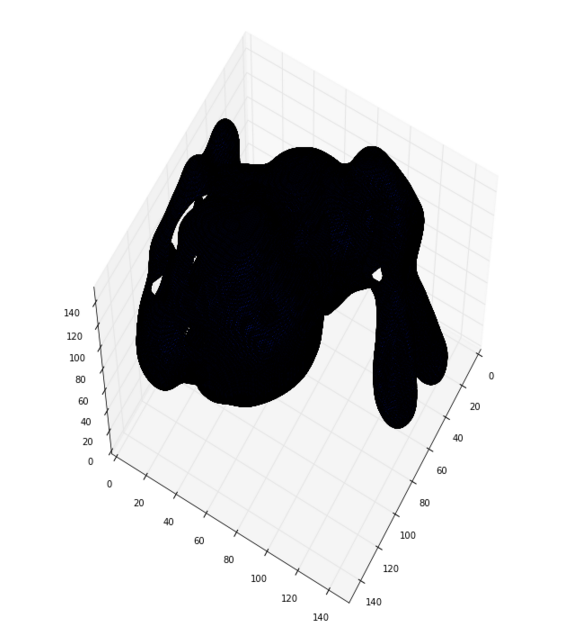
\includegraphics[scale=.5]{rabbit_marching.ps}\\
\\
We also plot a scatter plot of the level set to contrast.\\
Stanford Bunny:
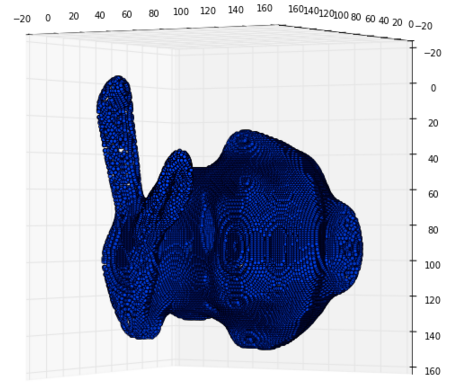
\includegraphics[scale=.6]{rabbit_scatter.ps}

We notice that as $\sigma$ grows, some eigenvalues of the Gram matrix move towards 0. These eigenvalues often can become negative due to machine precision, and then we cannot proceed with a non-positive semi-definite matrix.\\

We also implement incomplete Cholesky decomposition, but as this drops low eigenvalues, we again run into the same problem with non-positive semi-definite Kernel matrices due to machine precision.\\

We notice that as the data size grows, inverting the Hessian grows at $n^3$. To combat this, we can optimize with steepest descent or a Jacobian approximation. The trade off is of course that the descent takes longer to run since we're not taking advantage of quadratic convergence. \\
\\

\section{Conclusion}~\\

Scaling with large datasets is becoming more important as computing capacity grows. 
3D printers are also becoming more powerful and need accurate models to be useful.
Manipulating all of this data together, at once, is too taxing for hardware. Thus using more compact models is highly desirable for many of these applications. 


~\\
~\\
~\\
%%\newpage

\begin{thebibliography}{1}

\bibitem{Platt} {\sc B. Scholkopf, J. Platt, J. Shawe-Taylor, A. J. Smola, and R. C. Williamson.} Estimating the support of a high-dimensional distribution. {\em Neural Computation}, 13:1443?1471, 2001.

\bibitem{Tax} {\sc D. M. J. Tax and R. P. W. Duin.} Support vector data description. {\em Machine Learning}, 54:45?66, 2004.

\bibitem{Simon} {\sc Bernhard Sch�lkopf and Joachim Giesen and Simon Spalinger.} Kernel methods for implicit surface modeling. {\em Advances in Neural Information Processing Systems 17}, 1193-1200, 2005.

\bibitem{Jordan}{\sc Bach and Jordan.} Kernel Independent Component Analysis. {\em Journal of Machine Learning Research 3}, 1-48, 2002.

\bibitem{Fine}{\sc Fine and Scheinberg.} Efficient SVM Training Using Low-Rank Kernel Representations. {\em Journal of Machine Learning Research 2}, 243-264, 2001.

\bibitem{Jordan2}{\sc Bach and Jordan.} Predictive low-rank decomposition for kernel methods. {\em ICML '05}, 33 - 40, 2005.


\end{thebibliography}

\end{document}
